\section{Architecture overview}

The ABEL library can be splitted into a Frontend and a Backend part.
The frontend provides the main API, which is completely agnostic of the actual storage engine, 
whereas the backend provides a framework and some implementations to adapt ABEL to a specific storage engine.
The boundary between Backend and Frontend can be drawn straight through the deferred class REPOSITORY.

\subsection{Frontend}

If you've read the previos part of the documentation, then you should be quite familiar now with the frontend.
The main classes are:
 \begin{itemize}
  \item CRUD\_EXECUTOR: Provides features for CRUD operations, and does some error handling for transaction conflicts.
  \item QUERY: Collects information like the Criteria, Projection, and (through its generic parameter) the type of the object to be retrieved. It doesn't do anything by itself.
  \item TRANSACTION: Represents an ABEL transaction, and is responsible to internally propagate errors. It provides the features commit and rollback, but internally it relies on REPOSITORY to execute them.
  \item CRITERION: Its descendants provide a filtering function for retrieved objects, and it has builtin functions to generate a tree of criteria using the overloaded logical operators.
 \end{itemize}

You can see that the main objective of the frontend is to provide an easy to use, backend-agnostic API, and to collect information that the backend can consume.

\todo{Insert class diagram}


\subsection{Backend}

The frontend needs a repository which is specific to a data storage engine, and the backend provides a framework to implement these repositories (in cluster Framework).
There are also some already predefined repositories inside the backend (cluster Backends), like the IN\_MEMORY\_REPOSITORY.

Inside the framework, there are basically three layers of abstraction. The first is the deferred class REPOSITORY, which is still very object-oriented:
It takes Eiffel objects that may have a big object graph attached, and returns such fully loaded objects. 
It also provides some fine-grained control to restrict depth in an object graph.

The second important level of abstraction is the deferred class BACKEND\_STRATEGY, which deals only with one object at once. 
The layer in between REPOSITORY and BACKEND\_STRATEGY take care of disassembling the object graph into single objects, wrapped in a more explicit notion of the object graph. 
You can read in the object-relational mapping section ~\ref{section:ORM} how this is exactly done.
Anyway, the BACKEND\_STRATEGY only knows the concept of a single object and of a collection, and it is responsible to map these to the actual persistence mechanism, e.g. a database with a specific layout. 

The third layer of abstraction is a set of wrappers to a database. It only wraps the connection details, and has functions to execute SQL and retrieve the result in a standardized way.
It is very useful if you want to easily swap e.g. from a MySQL database to SQLite, but its abstraction is not perfect - i.e. it doesn't take into account the different SQL variations.

The most important data structure in the framework is the OBJECT\_\-IDENTIFICATION\_MANAGER: 
It maintains a weak reference to every object that has been queried or inserted before, and assigns a repository-wide unique number to it (called the object\_identifier).
It is, for example, responsible for the fact that the update fails in section ``Recognizing Objects''~\ref{subsection:recognize_objects}.

Another important datastructure is the KEY\_POID\_TABLE, which maps the objects object\_identifier to the primary key of the corresponding entry in the database.

To visualize the whole structure, there is a class diagram that shows the most important classes and concepts. You can also see two implementations of the backend abstraction there.

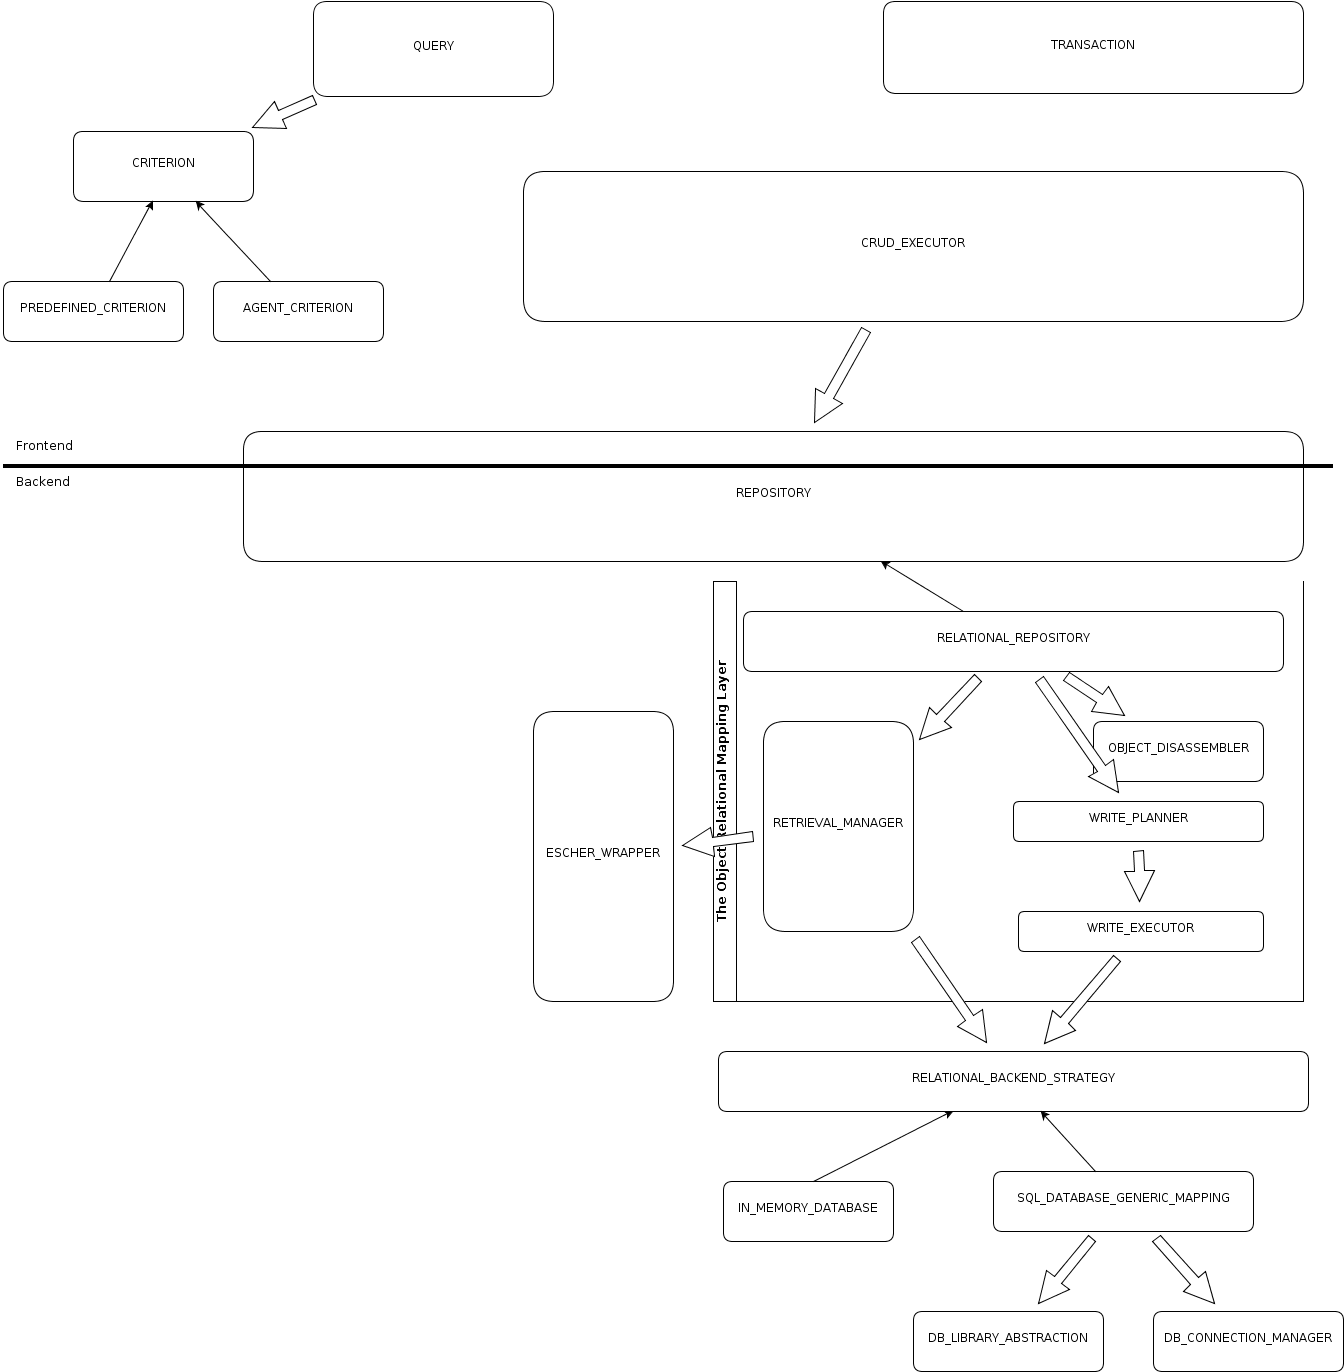
\includegraphics[width = 13cm] {class_diagram.png}

\section{Object-relational Mapping}
\label{section:ORM}

The object-relational mapping layer lies between the REPOSITORY and the BACKEND\_STRATEGY layer.
It mainly consists of four main classes doing the actual work, and a set of helper classes that represent an object graph.

The object graph representation classes are all in folder ``framework/object\_graph\_representation''. 
Although their main purpose is to represent an object graph, they are also used to describe a write operation (the BACKEND\_STRATEGY actually takes such objects as an argument)
These are the most important ones:

\begin{itemize}
 \item BASIC\_ATTRIBUTE\_PART represents an object of a basic type
 \item COLLECTION\_PART represents a collection, e.g. an instance of SPECIAL.
 \item SINGLE\_OBJECT\_PART: represets an Eiffel object that is neither a basic type nor a collection.
\end{itemize}

All these classes inherit from a deferred class OBJECT\_GRAPH\_PART. 
They have a builtin iteration cursor, and they share the concept of dependencies.
If an object graph part X is dependent on another part Y, then it means for example that Y has to be inserted first, because X needs its primary key as a foreign key in the database.

The four classes listed here are the ones that do the actual work:

\begin{itemize}
 \item The OBJECT\_DISASSEMBLER is responsible to create the explicit data structure for an object graph.
 \item The WRITE\_PLANNER is responsible to generate a total order on all write operations.
 \item The RETRIEVAL\_MANAGER builds objects from the parts that it gets from the backend, and takes care that all referenced objects of a retrieved object get loaded as well.
 \item The COLLECTION\_HANDLER, or rather its descendants, add collection handling support to the basic ORM layer. You need at least one handler for SPECIAL, but you can add handlers for other collection as well.
\end{itemize}

The object writing part is a bit more complex than the reading part, because of this dependency issue.


\todo{ Add a little visualization of the different parts}

\subsection{Collection handling}

You can extend the ORM algorithm to include collections. A collection is usually mapped differently from a normal object in the backend, e.g. through a M:N-relation table.
By default you need at least one handler for SPECIAL, because of its peculiarity that it doesn't have a fixed amount of fields.
But you can include any other collection, e.g. a LIST or an ARRAY.

There are two types of collections that you can create within a handler. 
The RELATIONAL\_COLLECTION is intended for a case when you have a typical database layout, with tables for a specific class and relations stored either with in the referenced object table (1:N-Relations) or inside their own table.
The OBJECT\_COLLECTION is intended for a scenario where you can store collections in a separate table, having their own primary key, and with the collection owner using this key as a foreign key.

It depends on the database layout of the backend which collection part you need to create.

\subsection{Object graph settings}

First, let's define the object graph more exactly, using graph theory.
A vertex in the graph corresponds to an object, and a reference is an edge.

The (global) object graph is the web of objects and references as it is currently in main memory.

An object Y can be ``reached'' from another object X if there is a path between X and Y, i.e. Y is in the transitive closure of X.

The object graph of an object X is the induced subgraph containing all vertices that can be reached from X.

The level of an object Y in the object graph of X is the length of the shortest path from X to Y.

Using these definitions we can now describe how ABEL handles object graphs, and how you can tweak the default settings to increase performance.

Every operation in ABEL has its own depth parameter (defined in OBJECT\_GRAPH\_SETTINGS), which has the following effect:
Each operation will only handle the objects when the following condition holds: $ level(object) < depth $

Now, let's put this in a known context:
You already know that the insert and retrieve features handle the complete object graph of an object. 
In fact, the depth for both functions is infinity by default.

On the other hand, the update or delete operations only handle first object they get, and don't care about the object graph.
Their depth is defined as exactly 1, which means that only an object with a level of 0 satisfies the condition above.
The only object with level 0 is in fact the root object of the object graph.

To fully understand the behaviour of ABEL, we also have to look at what happens when the algorithm reaches the ``last'' object, i.e. when the condition $level + 1 = depth$ holds.
In that case the object with all basic attributes gets inserted/updated, but references only get written if the referenced object is already persistent.
If it isn't persistent, then in a later retrieval operation the reference will be Void.

You can change the depth of the individual operations in REPOSITORY.default\_object\_graph. 
Please keep in mind that this is a dangerous operation, as a not fully retrieved or inserted object will contain Void references even in a void-safe environment, and it's also possible that they violate the invariant.

Apart from the depth, there are some other settings as well, i.e. what ABEL should do if it finds an already persistent object along the object graph of a new object to insert, or vice versa.

\section{Backend abstraction}


\subsection{REPOSITORY}

\subsection{BACKEND\_STRATEGY}

\subsection{Database wrapper}


\section{Extensions}

\section{Adaption to a specific database layout}


\section{Limitations of the library}
TODO

Current limitations:
\begin{itemize}
\item Not all features available if adapted to a custom DB layout 
\item Inheritance currently not properly supported (due to limitation of INTERNAL)
\item Reals have rounding error
\item No ordering support (at least not yet)
\item
\end{itemize}

%What exactly has to be here? Is a missing feature (like ordering support) a limitation as well?


TODO

%\section{ PART 2: Technical Documentation}

%\subsection{Moved to technical documentation}
%about criteria
%It will internally build a tree of criteria, with specialized AND, OR or NOT instances as nodes and the usual predefined or agent instances as leafs.


%\subsubsection{Performance remarks}

%ABEL will try to let the backend do as much of the filtering as is possible, to reduce the overhead of e.g. network communication or building unnecessary objects.
%This especially means that ABEL will compile predefined queries to SQL if you have a relational database as a backend. 
%However, if there is an agent criterion OR-ed to a predefined criterion, the test can not be made in the database because you might get false negatives.
%Therefore, to have optimal performance, you should consider the following points:

%\begin{itemize}
%\item Try not to use agent criteria if you have a relational database backend.
%\item Try not to use OR on agent criteria.
%\item Try to keep OR-ed agent criteria as deep down the tree as possible (as the above OR-node defaults to true and thus is not checked for in the backend)
%\end{itemize}
